% Permission is granted to copy, distribute and/or modify this document
% under the terms of the GNU Free Documentation License, Version 1.3
% or any later version published by the Free Software Foundation;
% with no Invariant Sections, no Front-Cover Texts, and no Back-Cover Texts.
% A copy of the license is included in the section entitled "GNU
% Free Documentation License".
%
% Authors:
% Caner Candan <caner@candan.fr>, http://caner.candan.fr

% TODO
% faire un nouveau plan
% pour fin mai: comparaison et description des expériences et description des scripts

\newcommand {\copyleft}
{%
  \lang{%
    Permission is granted to copy, distribute and/or modify this document under the terms of the GNU Free Documentation License, Version 1.3 or any later version published by the Free Software Foundation; with no Invariant Sections, no Front-Cover Texts, and no Back-Cover Texts. A copy of the license is included in the section entitled "GNU Free Documentation License". The sources may be freely downloaded, used and modified from the url {\tt https://github.com/canercandan/msc-thesis}.%
  }{%
    Ce papier suit les termes de la licence ``GNU Free Documentation License 1.3'' et peut être librement téléchargé, utilisé et modifié depuis l'url {\tt https://github.com/canercandan/msc-thesis}.%
  }%
}

\newcommand {\thales} {{\tt Thales Research \& Technology}}

\title{%
  \lang{%
    {\bf Optimizations using stockastic algorithms\\and high performance computing}\\{\em MSc Thesis}%
  }{%
    {\bf Optimisations basées sur des algorithmes stochastiques\\et calcul à haute performance}\\{\em Mémoire pour l'obtention du titre de Master}%
  }%
  \footnote{\copyleft}
}

\begin{document}

\maketitle

\begin{abstract}

  Written during my internship at \thales, this thesis illustrates the following topics: Parallelization of a planning algorithm using EO framework on a 48-core machine, experiments showed significant speedups with an increasing number of cores – Hybridation of EDA \& SA – Implementation of an automated parameter setting interface.

\end{abstract}

\section{\lang{Aknowledgement}{Remerciements}}

\lang{
  I cannot begin writting this thesis without sincerely thanking all who have helped as much as they could while this extremely rich experience.
}{
  Je ne pourrais commençais la rédaction de ce mémoire sans remercier sincèrement toutes les personnes qui m'ont aidées de près ou de loin durant cette expérience extrêmement riche.
}

\section{Introduction}

\paragraph{\lang{Evolutionary algorithms}{Les algorithmes évolutionnistes}}

\lang{
  Ranked among computational intelligence methods, a domain close to artificial intelligence, the evolutionary algorithms are mainly inspired by the theory of evolution.
  In order to produce the best results to a given problem, they evolve a set of solutions.
  % introduce notion of local and global optimum
  There stochastic nature is due to the iteratively use of random processes.
  Also known as ``metaheuristics'', the vast majority of these methods are used to solve optimization problems.
}{
  Les algorithmes évolutionnistes forment une famille d'algorithmes. Inspirés par la théorie de l'évolution, ils résouent une variété de problèmes. Ils font évoluer un ensemble de solutions pour un problème donné afin d'obtenir les meilleurs résultats. Leur particularité stochastique est dû à l'utilisation, itératif, de processus aléatoires. Aussi connu sous le nom de ``métaheuristiques'', la grande majorité de ces méthodes sont utilisées pour résoudre des problèmes d'optimisation. Ils sont classés parmi les méthodes d'intelligence informatiques, un domaine proche de l'intelligence artificielle.
}

\begin{figure}[H]
  \centering
  \includegraphics[scale=0.5]{images/evolutionary_algorithm_scheme}
  \caption{The steps of an evolutionary algorithm}
\end{figure}

% \begin{figure}[H]
%   \centering
%   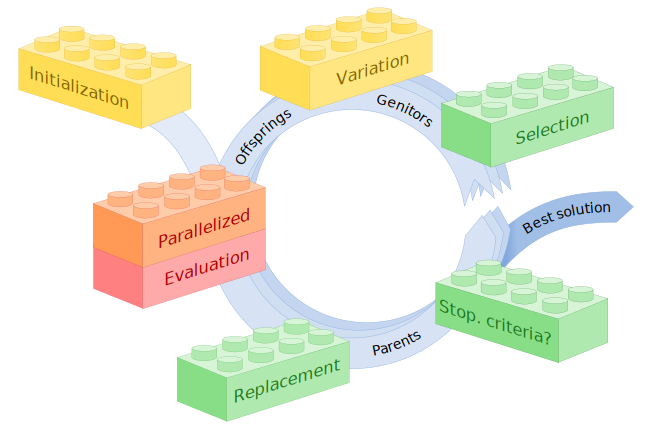
\includegraphics[scale=0.5]{images/evolutionary_algorithm_scheme_parallel}
%   \caption{The steps of an evolutionary algorithm including parallelized evaluation}
% \end{figure}

\paragraph{\lang{High performance computing}{Calcul haute performance}}

Since the emergence of processors, the manufactors have produced more and more fast architectures by increasing the clock rate. Thereby the performances of programs are enhanced without needing any modifications. Defined by the Moore law, this method had to normaly persist to 2015. But by growing the clock rate it also increases the head disspation. 2004 was the year of an important failover. We were progressively switching to processors with several computational cores and the developers were facing a new conception way: closer to metal.

\section{\lang{Evolving Objects Framework}{Le framework EO}}

\lang{
  With the help of EO, you can easily design evolutionary algorithms that will find solutions to virtually all kind of hard optimization problems, from continuous to combinatorial ones.
}{
  A l'aide du framework EO, il devient possible de concevoir facilement et intuitivement des algorithmes évolutionnistes qui trouveront des solutions à tous les genres de problème virtuel en optimisation difficile allant de l'optimisation continue au combinatoire.
}

\section{Parallelization of an evolutionary algorithm}

\begin{figure}[H]
  \centering
  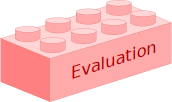
\includegraphics[scale=0.5]{images/evaluation_box}
  %\caption{The steps of an evolutionary algorithm}
\end{figure}

\begin{figure}[H]
  \centering
  \includegraphics[scale=0.5]{images/parallelized_evaluation_boxes}
  %\caption{The steps of an evolutionary algorithm}
\end{figure}

\section{Parallelization and Scalability}

In order to speed the parallelization up, we had to be careful about the scalability of the framework. Indeed for small population sizes the work (efficiency) of the processors is roughly closed to 100\% but for sizes bigger than 100 individuals we observe a speed down of this processors' work. Usually, and using a data parallelization paradigm, the reason why the framework is not scalable is due to memory allocations which are not under control. One solution which solves this issue was to remove or replace all calls to the functions affecting the memory capacity of the main parents and offspring vectors (swap, ...).

\paragraph{Incremental memory allocation issue}

As we are working in a parallel version of EO as well as minimizing the time consuming, we have found this issue doing incremental allocations in the variation operator's classes.

\bibliographystyle{abbrv}
\begin{thebibliography}{10}

\bibitem{dae:gecco2011}
C. Candan, J. Dr{\'e}o, P.~Sav\'eant and V.~Vidal.
\newblock {Parallel Divide-and-Evolve: Experiments with OpenMP on a Multicore Machine}.
\newblock In {\em $21^{st}$ Genetic and Evolutionary Computation Conference (GECCO'11)}, pages XXX--XXX. ACM Press, 2011.

\bibitem{edasa:roadef2011}
J. Dr{\'e}o, C. Candan.
\newblock {Hybride d'algorithme à estimation de distribution et de recuit simulé pour l'optimisation continue}.
\newblock In {\em $12^{th}$ Société française de Recherche Opérationnelle et d’Aide à la Décision (ROADEF'11)}, 2011.

\end{thebibliography}

\end{document}


% \section{ParadisEO}

% % look at http://paradiseo.gforge.inria.fr/index.php?n=About.Publi

% \section{\lang{Parallelization on a distributed environment using PEO}{Paraléllisation dans un environnement distribué en utilisant PEO}}

% \section{\lang{An hybrid algorithm in estimating of distribution parameters and simulated annealing for continuous optimization}{Hybride d'algorithme à estimation de distribution et de recuit simulé pour l'optimisation continue}}

% \section{Parallélisation de la recherche de fronts de performances pour le paramétrage de métaheuristiques}

% \section{\lang{Parallel Divide-and-Evolve: Experiments with OpenMP on a Multicore Machine}{Divide-and-Evolve en parallèle: expérimentation avec OpenMP dans un environnement multi-coeurs}}

% \section{Conclusion}
